\documentclass[./\jobname.tex]{subfiles}
\begin{document}
\chapter {Experiment 0: Serial Memetic JADE}
\label{chap:experimet_0}

This chapter describes the results obtained by the most basic adaption of JADE for solving \gls{pde}s. The algorithm used here, builds on the concepts described in \cite{chaquet_using_2019}. Aside from substituting some parameters, the only main difference is the usage of JADE instead of a \gls{cma_es}. 

\section{Hypotheses}
A memetic algorithm was first mentioned by \cite{moscato_evolution_2000}. In essence, it is a hybridisation of a population-based evolutionary algorithm and a deterministic direct or local search. The pseudocode \ref{algo: memeticJADE} below shows the implementation of such a memetic JADE. At first, JADE performs the global search and places its population around the optimum. Than the \gls{ds} exploits this area. The budget of \gls{nfe} is split into two parts: JADE takes nearly all \gls{nfe} and leaves $2\cdot dim$ \gls{nfe} for the \gls{ds}. 

\begin{algorithm}[h]
	\SetAlgoNoLine
	\DontPrintSemicolon
	\SetKwFunction{FmJADE}{memeticJADE}
	\SetKwProg{Fn}{Function}{:}{}
	\Fn{\FmJADE{$\mathbf{X}$, $funct$, $minErr$, $maxFE$}}{
		$dim$, $popsize$ $\gets size(\mathbf{X})$\;
		$p \gets 0.3$\;
		$c \gets 0.5$\;
		$pop$, $FE$, $F$, $CR$ $\gets JADE($$\mathbf{X}$, $p$, $c$, $funct$, $minErr$, $maxFE - 2 dim$ $)$\;
		$bestIndex = argmin(FE)$\;
		$bestSol = pop[bestIndex]$\;
		$pop$, $FE$ $ = downhill\text{ }simplex($$funct$, $bestSol$, $minErr$, $2 dim)$\;
		\Return $pop$, $FE$, $F$, $CR$
	}
	\unterschrift{memetic JADE Pseudocode}{}{}
	\label{algo: memeticJADE}
\end{algorithm}

This experiment provides first insight into the performance of the proposed algorithm. It tries to answer the question, if JADE is a suitable surrogate algorithm for a \gls{cma_es}. Further, the memory usage and solving time is compared to the \gls{fem} results obtained in chapter \ref{chap:fem_baseline_results}. 

\section{Experiment Setup}
The standard parameters from table \ref{tab:ci_parameter} are taken. The memetic JADE is limited to either $10^4$ \gls{nfe} or $10^6$ \gls{nfe}. The experiment is done on two different machines. The first try with $10^4$ \gls{nfe} is run on the same machine ($\rightarrow$ machine 1) as the \gls{fem} experiment. This allows for a fair memory and solving time comparison. This comparison can not be performed with the data obtained by using $10^6$ \gls{nfe} ($\rightarrow$ machine 2). Further, 5 \gls{gak} are used which results in a dimension of 20 parameters. Thus, the population consists of 40 individuals. 

\section{Result}
\label{chap:experimet_0_results}
Table \ref{tab:results_literature_comparison} shows a comparison on the common testbed functions \gls{pde} 2 and \gls{pde} 3 with numerical results obtained in other research papers. It is important to notice, that the parameters, used to obtain the results, might not coincide. \cite{tsoulos_solving_2006} also use these two \gls{pde}, but their paper did not provide any usable error metric. 
\begin{table}[H]
	\centering
	\noindent\adjustbox{max width=\linewidth}{
		\begin{tabular}{|c|c|c|c|}
			
			\hline
			\rowcolor[HTML]{\farbeTabA}
			
			Paper & parameter & RMSE \gls{pde} 2 & RMSE \gls{pde} 3 \\ \hline
			\cite{chaquet_using_2019} & \multilinecell{4 kernel \\ max \gls{nfe}=$10^6$ \\ 50 replications } & $(1.75 \pm 1.14) 10^{-4}$ & $(1.09 \pm 0.846) 10^{-5}$  \\ \hline
			\cite{chaquet_solving_2012} & \multilinecell{10 harmonics \\ max \gls{nfe} = $G \cdot \lambda$ = $1.2 \cdot 10^6$ \\ 10 replications} & $(6.37 \pm 0.733) 10^{-3}$ & $(5.90 \pm 0.799)10^{-3}$ \\ \hline
			\cite{sobester_genetic_2008}& \multilinecell{50 max tree lenght \\ 12 generations \\ 20 replications} & $(6.9 \pm 8.3)10^{-4}$ & --X-- \\ \hline
			\cite{panagant_solving_2014}& \multilinecell{unknowns: N/A \\ \gls{nfe}=$5\cdot 10^5$ \\ replications: N/A} & $7.256 10^{-4}$ & $9.489 10^{-6}$ \\ \hline
			serial memetic JADE & \multilinecell{5 kernel \\ max \gls{nfe} = $10^6$ \\ 20 replications} & $(2.9798 \pm 1.5541)10^{-2}$ & $(3.8225 \pm 1.9438)10^{-2}$ \\ \hline
			
		\end{tabular}
	}
	\unterschrift{This table compares the results obtained with the serial memetic JADE to the numerical results obtained by similar work in literature. The same metric must be used, thus the RMSE as defined in equation \ref{eq:rmse_chaquet} is calculated.}{}{}
	\label{tab:results_literature_comparison}
\end{table}

The following table \ref{tab:serial_jade_compare_10^6_10^4} lists the smallest L2 norm reached after $10^4$ \gls{nfe} and $10^6$ \gls{nfe}, respectively. A standard Wilcoxon test, as described in \ref{chap:software_architecutre}: post processing, is performed. Remarkable is that on \gls{pde} 5, more \gls{nfe} result in a significantly worse solution.  

\begin{table}[H]
	\centering
	\noindent\adjustbox{max width=\linewidth}{
		\begin{tabular}{|c|c|c|c|c|l|}
			
			\hline
			\rowcolor[HTML]{\farbeTabA}
			
			\gls{nfe} & \multicolumn{2}{|c|}{$10^4$} & \multicolumn{2}{|c|}{$10^6$} & \\ \hline
			stat & mean & median & mean & median & Wilcoxon Test \\ \hline \hline
			\gls{pde} 0A & 1.9415 $\pm$ 0.3321 & 1.8844 & 0.6596 $\pm$ 0.5510 & 0.9285 & sig. better \\ \hline
			\gls{pde} 0B & 0.7137 $\pm$ 0.1979 & 0.6354 & 0.2027 $\pm$ 0.1302 & 0.1516 & sig. better \\ \hline
			\gls{pde}  1 & 0.1874 $\pm$ 0.0408 & 0.1938 & 0.0149 $\pm$ 0.0049 & 0.0151 & sig. better \\ \hline
			\gls{pde}  2 & 0.0890 $\pm$ 0.0334 & 0.0760 & 0.0257 $\pm$ 0.0140 & 0.0224 & sig. better \\ \hline
			\gls{pde}  3 & 0.2409 $\pm$ 0.1051 & 0.2309 & 0.0328 $\pm$ 0.0169 & 0.0285 & sig. better \\ \hline
			\gls{pde}  4 & 0.1102 $\pm$ 0.0367 & 0.0985 & 0.0378 $\pm$ 0.0083 & 0.0352 & sig. better \\ \hline
			\gls{pde}  5 & 0.6645 $\pm$ 0.1930 & 0.6263 & 1.1968 $\pm$ 0.0286 & 1.2056 & sig. worse \\ \hline
			\gls{pde}  6 & 1.9660 $\pm$ 1.3845 & 1.6540 & 0.4135 $\pm$ 1.2133 & 0.0018 & sig. better \\ \hline
			\gls{pde}  7 & 0.0457 $\pm$ 0.0137 & 0.0452 & 0.0221 $\pm$ 0.0019 & 0.0223 & sig. better \\ \hline
			\gls{pde}  8 & 0.2186 $\pm$ 0.0045 & 0.2191 & 0.2170 $\pm$ 0.0019 & 0.2175 & unsig. better \\ \hline
			\gls{pde}  9 & 0.0525 $\pm$ 0.0147 & 0.0516 & 0.0451 $\pm$ 0.0119 & 0.0459 & unsig. better \\ \hline
			
		\end{tabular}
	}
	\unterschrift{L2 norm reached with serial JADE at $10^4$ \gls{nfe} and $10^6$ \gls{nfe}}{}{}
	\label{tab:serial_jade_compare_10^6_10^4}
\end{table}

The following two images \ref{fig:serial_jade_time_boxplot} and \ref{fig:serial_jade_memory_boxplot} show the time and memory usage for solving the testbed with $10^4$ \gls{nfe}. The images highlight the varying complexity of the testbed-\gls{pde}s and their corresponding fitness function. Although these results are not obtained for $10^6$ \gls{nfe}, they provide insight on how the solver scales with more \gls{nfe}. 

\begin{figure}[H]
	\centering
	\noindent\adjustbox{max width=0.66\linewidth}{
		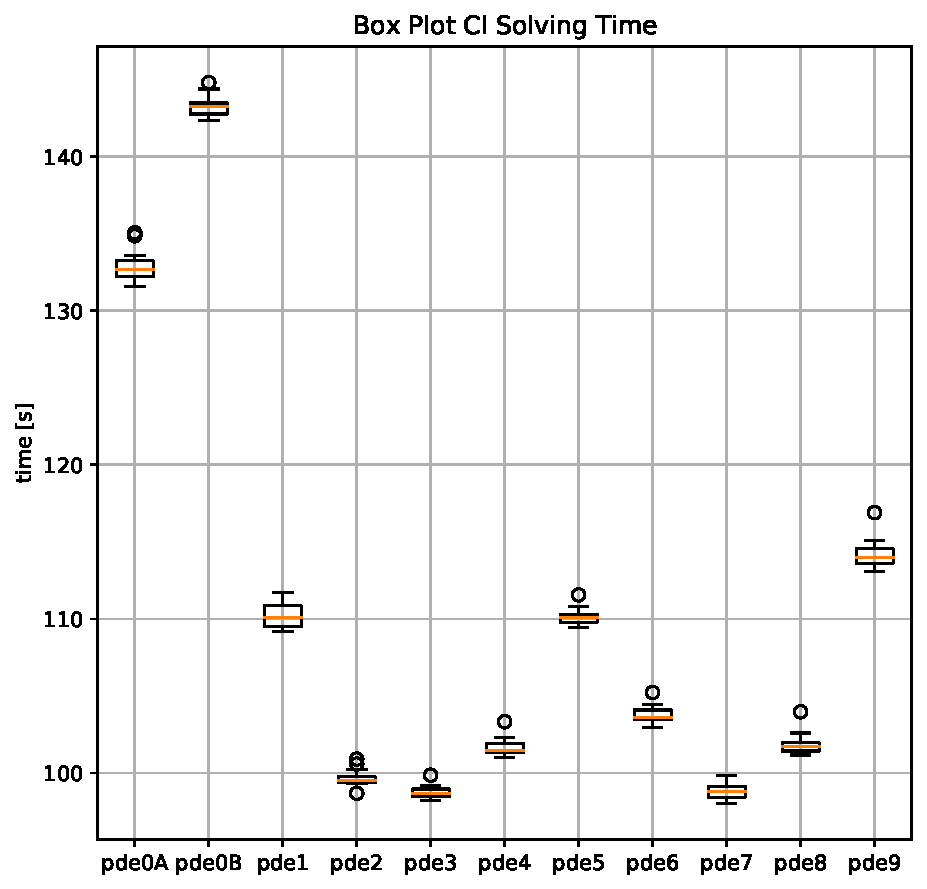
\includegraphics[width=\textwidth]{../../code/experiments/experiment_0/time_boxplot_ci_exp0.pdf}
	}
	\unterschrift{Solving time at $10^4$ \gls{nfe}.}{}{}
	\label{fig:serial_jade_time_boxplot}
\end{figure}


\begin{figure}[H]
	\centering
	\noindent\adjustbox{max width=0.66\linewidth}{
		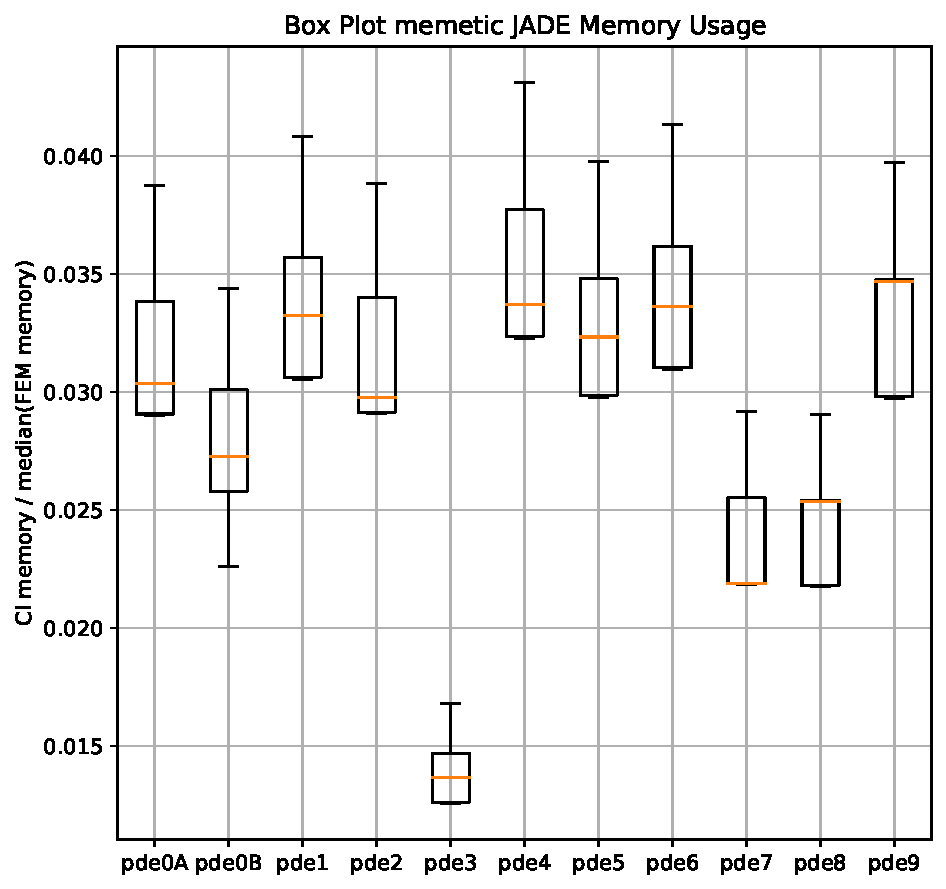
\includegraphics[width=\textwidth]{../../code/experiments/experiment_0/mem_boxplot_ci_exp0.pdf}
	}
	\unterschrift{Memory usage with $10^4$ \gls{nfe}.}{}{}
	\label{fig:serial_jade_memory_boxplot}
\end{figure}

\section{Discussion}

The results presented in the chapter \ref{chap:experimet_0_results} above, are discussed on the following pages. 

\subsection{Comparison to Literature}

The \gls{rmse} reached on the \gls{pde} 2 and 3, are clearly not as good as the results obtained in previous work, especially the results presented in \cite{chaquet_using_2019}. There might be three reasons for that: 
\begin{itemize}
	\item As stated in the previous table \ref{tab:ci_parameter}, the penalty and weighting factor on the collocation points are different. Further, more kernels are used, resulting in a greater search dimension while simultaneously using a smaller population size. The combination of these parameters might influence the quality of the solution to the worse. 
	\item Compared to \cite{chaquet_using_2019}, the \gls{nfe}-budget for the local \gls{ds} search is smaller, thus the exploitation might not be as progressed.
	\item JADE might simply be not as well suited for the problem as a \gls{cma_es}. 
\end{itemize}


%%%%%%%%%%%%%%%%%%%%%%%%%
%        time/mem       %
%%%%%%%%%%%%%%%%%%%%%%%%%

\subsection{Time/Memory Usage}

The results from table \ref{tab:serial_jade_compare_10^6_10^4} show, that the \gls{ci} solver can not nearly compete with the results obtained by the \gls{fem} solver from table \ref{tab:fem_sol_quality}. 
However, more interesting is the comparison of time and memory usage. 
In the current implementation, the population, the corresponding function values as well as the F and the CR history are recorded at every generation. This is not necessary for the performance of the algorithm, but helpful for evaluating the results. Therefore, the memory usage scales linearly with the number of function evaluations used $\mathcal{O}(n)$. In later implementation, this could be disregarded to further reduce the memory consumption. Every \gls{pde} takes about the same amount of memory to solve, somewhere between 1.5 and 2.2 Mbyte. 
The \gls{ci} solver takes somewhere between 100 and 150 seconds (figure \ref{fig:serial_jade_time_boxplot}) to perform $10^4$ \gls{nfe}, depending on the \gls{pde} problem. This is always longer than the \gls{fem} solver, with the exception of \gls{pde} 3. More importantly, the \gls{ci} solver uses less memory, on all problems(figure \ref{fig:serial_jade_time_boxplot}). An interesting observation is the distribution of the solving time within the testbed. The more commands a fitness function needs, the longer is its solving time. However, this does not necessarily correspond with the quality of the solutions. For example, \gls{pde} 0B takes the longest to evaluate but, compared to the other \gls{pde}s, it reaches a ``fairly'' good quality. 


%%%%%%%%%%%%%%%%%%%%%%%%%
%         PDE0A         %
%%%%%%%%%%%%%%%%%%%%%%%%%

\subsection{PDE 0A}
\label{chap: experiment_0_pde_0A}

The purpose of this \gls{pde} was to show that the solver would converge globally towards the analytical solution, if it could be represented by a finite number of kernels. Unfortunately, this can not be confirmed with the current implementation. While more function evaluation do tend to generate better results (as confirmed by the Wilcoxon test in table \ref{tab:serial_jade_compare_10^6_10^4}), it is not uncommon for the \gls{ci} solver to result in different functions. A typical phenomenon is to miss out some of the five Gauss bumps, that build the solution. The comparison of two solutions with $10^4$ \gls{nfe} and $10^6$ \gls{nfe} in figure \ref{fig:serial_jade_pde0a_sol_comparison} shows this behaviour. Since the results do get a lot better from $10^4$ to $10^6$ \gls{nfe}, it is possible that the results from $10^6$ \gls{nfe} can be improved. However, this is not tested due to the already extensive amount of computational effort. 

\begin{figure}[H]
	\centering
	\begin{subfigure}[b]{0.5\linewidth}
		\centering
		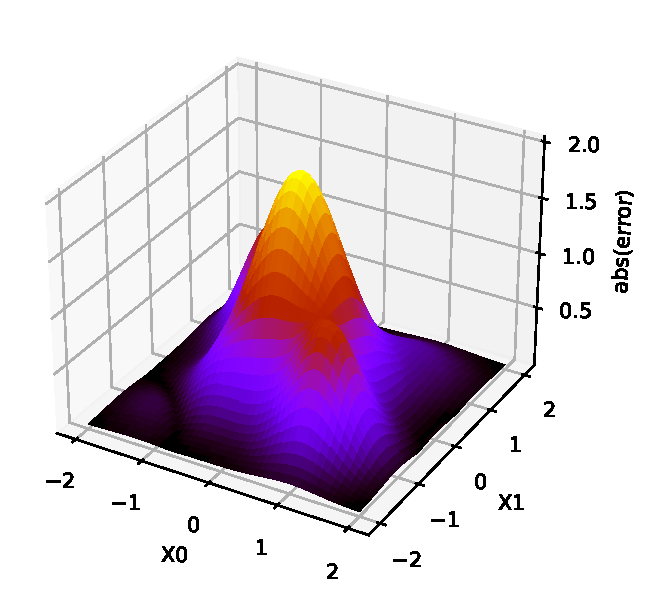
\includegraphics[width=1\textwidth]{../../code/experiments/experiment_0/pde0a_missing_bump_sol_10_4.pdf}
		\caption{\gls{pde} 0A solution with $10^4$ \gls{nfe}: \\ L2 norm: 2.5074851055301095 \\ FE value: 4.412933901588106 \\ RMSE: 0.5699084204927098}
		\label{fig:pde0a_sol_10_4}
	\end{subfigure}% 
	%
	\begin{subfigure}[b]{0.5\linewidth}
		\centering
		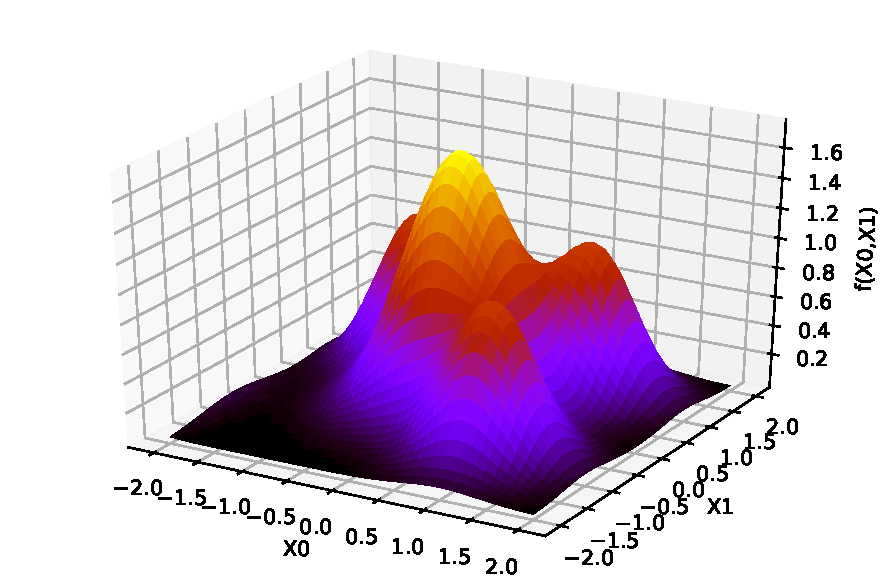
\includegraphics[width=1\textwidth]{../../code/experiments/experiment_0/pde0a_missing_bump_sol_10_6.pdf}
		\caption{\gls{pde} 0A solution with $10^6$ \gls{nfe}: \\ L2 norm: 0.9281243032816127 \\ FE value: 1.3761997083143358 \\ RMSE: 0.21103944621679302}
		\label{fig:pde0a_sol_10_6}
	\end{subfigure}%
	\unterschrift{Comparison of two typical \gls{pde} 0A solutions. }{}{}%
	\label{fig:serial_jade_pde0a_sol_comparison}
\end{figure}

\subsection{PDE 5}

%%%%%%%%%%%%%%%%%%%%%%%%%
%         PDE5          %
%%%%%%%%%%%%%%%%%%%%%%%%%
A fascinating property of \gls{pde}5 is observed: more function evaluation (from $10^4$ to $10^6$) result in a significantly worse solution quality. This is confirmed by a Wilcoxon test, as seen in the table \ref{tab:serial_jade_compare_10^6_10^4}. The corresponding histograms for the distribution of the L2 norm and the fitness value are depicted in figure \ref{fig:pde5_histograms}. 
A comparison of the best solution after $10^4$ \gls{nfe} and the best solution after $10^6$ \gls{nfe} is shown in the figure \ref{fig:serial_jade_pde5_sol_comparison}. This can also be concluded from a visual perspective: the solution after $10^4$ \gls{nfe} describes the global structure better. It seems, that the correct description of the boundary points becomes less important when more \gls{nfe} are allowed. This phenomenon can be explained by the structural difference between the fitness function and the L2 norm. The fitness of a candidate solution can only decrease or stay the same, thanks to the greedy selection used in JADE (line 15 in the pseudocode \ref{algo: jade}). Because the L2 norm is not the property that gets optimised, the quality of an individual at every generation is not necessarily monotonically decreasing. In the present case, this means that the fitness value does decrease, while the quality attribute gets worse, as confirmed by both histograms in figure \ref{fig:pde5_histograms}. 
This indicates, that a fundamental different strategy might be needed to obtain better results. 

\begin{figure}[H]
	\centering
	\begin{subfigure}[b]{0.5\linewidth}
		\centering
		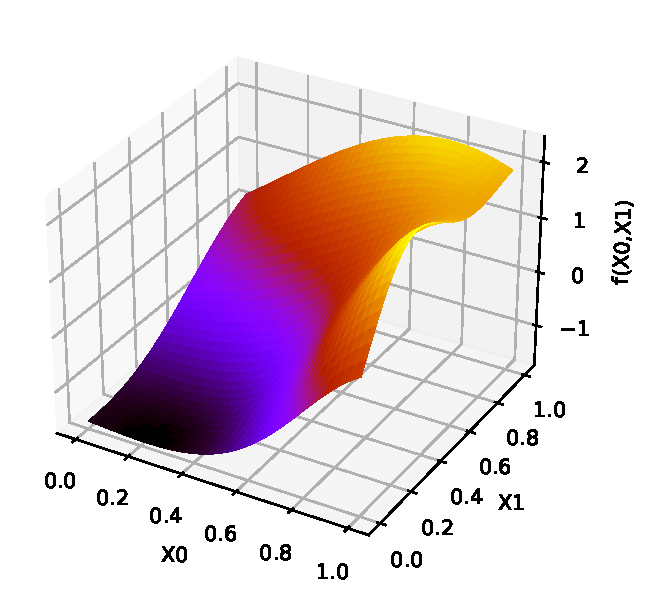
\includegraphics[width=1\textwidth]{../../code/experiments/experiment_0/pde5_best_sol_10_4.pdf}
		\caption{\gls{pde} 5 solution with $10^4$ \gls{nfe}: \\ L2 norm: 0.4283407099978464 \\ FE value: 2980.960124159222 \\ RMSE: 0.4648836893027784 }
		\label{fig:pde5_sol_10_4}
	\end{subfigure}% 
	%
	\begin{subfigure}[b]{0.5\linewidth}
		\centering
		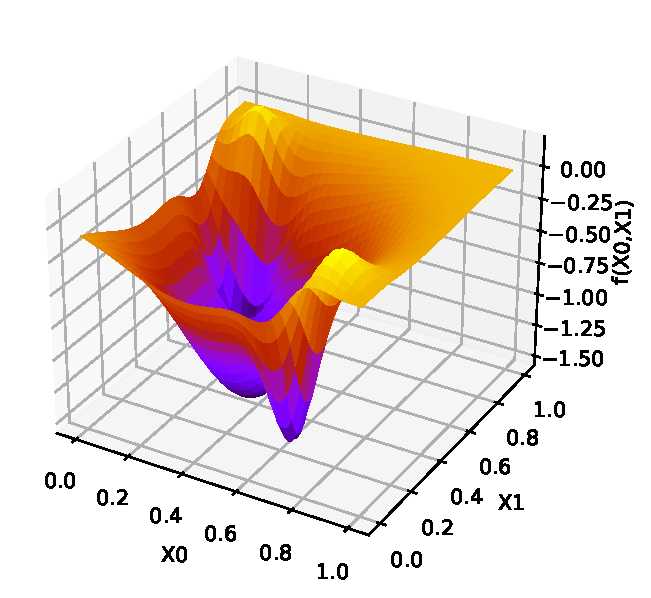
\includegraphics[width=1\textwidth]{../../code/experiments/experiment_0/pde5_best_sol_10_6.pdf}
		\caption{\gls{pde} 5 solution with $10^6$ \gls{nfe}: \\ L2 norm: 1.1095483876690175 \\ FE value: 1007.4408576392331 \\ RMSE: 1.1456143814668234 }
		\label{fig:pde5_sol_10_6}
	\end{subfigure}%
	\unterschrift{Comparison of the best achieved quality (fitness function, L2 norm and \gls{rmse}) solution on \gls{pde} 5}{}{}%
	\label{fig:serial_jade_pde5_sol_comparison}
\end{figure}



\begin{figure}[H]
	\centering
	\begin{subfigure}[b]{0.5\linewidth}
		\centering
		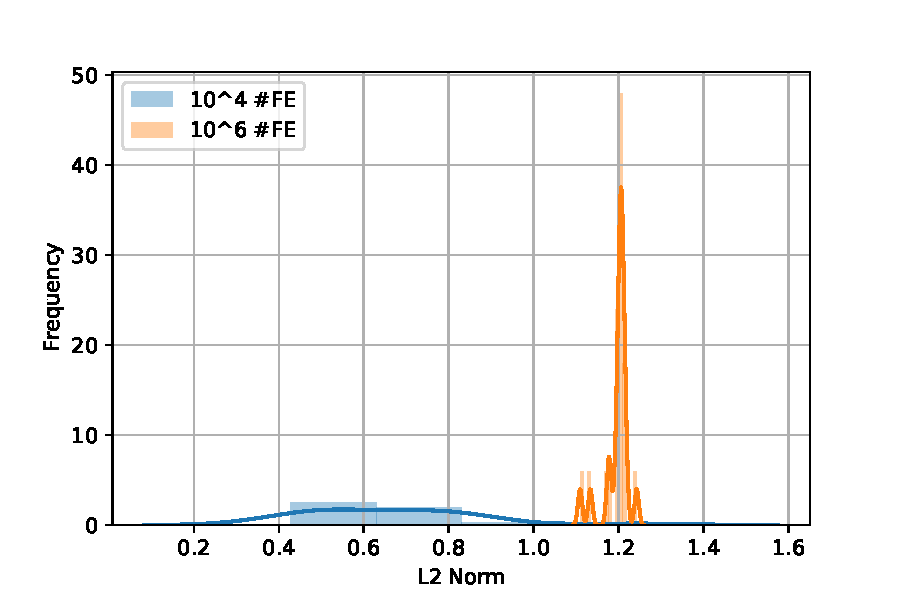
\includegraphics[width=1\textwidth]{../../code/experiments/experiment_0/pde5_norm_histogram.pdf}
		\caption{Histogram of the L2 norm reached on \gls{pde} 5.}
		\label{fig:pde5_norm_histogram}
	\end{subfigure}% 
	%
	\begin{subfigure}[b]{0.5\linewidth}
		\centering
		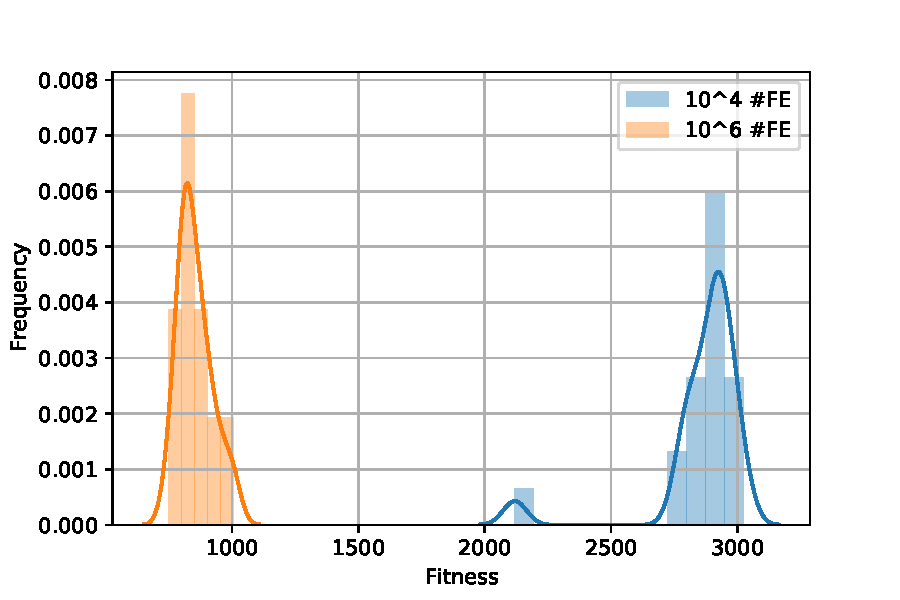
\includegraphics[width=1\textwidth]{../../code/experiments/experiment_0/pde5_fit_histogram.pdf}
		\caption{Histogram of the fitness value reached on \gls{pde} 5.}
		\label{fig:pde5_fitness_histogram}
	\end{subfigure}%
	\unterschrift{Histograms of the results reached with $10^4$ \gls{nfe} and $10^6$ \gls{nfe} on \gls{pde} 5. The paradox observation: the fitness value with $10^6$ \gls{nfe} is smaller, but the L2 norm tends to be larger. }{}{}%
	\label{fig:pde5_histograms}
\end{figure}

\end{document}